% ------------------------------------------------------------------------------
% TYPO3 CMS 6.2 LTS - What's New - Chapter "In-Depth Changes" (French version)
%
% @author	Paul Blondiaux <pblondiaux@sodifrance.fr>
% @author	Philippe Herault <philippe.herault@plan-net.fr>
% @license	Creative Commons BY-NC-SA 3.0
% @link		http://typo3.org/download/release-notes/whats-new/
% @language	French
% ------------------------------------------------------------------------------
% Chapter: In-Depth Changes
% ------------------------------------------------------------------------------

\section{In-Depth Changes}
\begin{frame}[fragile]
	\frametitle{Changements en profondeur}

	\begin{center}\huge{Chapitre 6 :}\end{center}
	\begin{center}\huge{\color{typo3darkgrey}\textbf{Changements en profondeur}}\end{center}

\end{frame}

% ------------------------------------------------------------------------------
% normalize.css
% ------------------------------------------------------------------------------
% http://forge.typo3.org/issues/47920

\begin{frame}[fragile]
	\frametitle{Changements en profondeur}
	\framesubtitle{Normalize.css}

	\begin{itemize}
		\item L'interface utilisateur Backend utilise \texttt{normalize.css}, ce qui rend tous les éléments plus cohérents et conformes aux standards actuels
		\item Moderne, compatible HTML5, alternative au traditionnel \textsf{CSS reset}
		\item Les objectifs de \texttt{normalize.css} sont :

			\begin{itemize}
				\item Préserver les comportements utiles par défaut des navigateurs plutôt que de les effacer
				\item Normaliser les styles pour de nombreux éléments HTML
				\item Corriger les bugs et les incohérences usuelles entre les navigateurs
				\item Améliorer légèrement l'utilisabilité
				\item Expliquer le code en utilisant les commentaires et une documentation détaillée
			\end{itemize}

	\end{itemize}

\end{frame}

% ------------------------------------------------------------------------------
% displayCond options BIT and !BIT
% ------------------------------------------------------------------------------
% http://forge.typo3.org/issues/45514

\begin{frame}[fragile]
	\frametitle{Changements en profondeur}
	\framesubtitle{TCA : Options displayCond BIT et !BIT}

	\lstset{
		basicstyle=\tiny\ttfamily
	}

	\begin{itemize}
		\item Vérifier à l'aide d'un champ multivaluée dans \texttt{displayCond} (bit à bit)\newline
			\texttt{BIT}: le bit est défini, \texttt{!BIT}: le bit \underline{n'}est \underline{pas} défini
	\end{itemize}

	\begin{columns}[T]

		\begin{column}{.5\textwidth}

			\advance\leftskip+1cm
			En supposant ce TCA :

			\lstset{xleftmargin=1cm}

			\begin{lstlisting}
				'content' => array(
				  'label' => '...',
				  'config' => array(
				    'type' => 'check',
				    'items' => array(
				      array('Content A', ''),
				      array('Content B', ''),
				      array('Content C', ''),
				    ),
				  )
				),
			\end{lstlisting}

		\end{column}
		\begin{column}{.5\textwidth}

			Exemples :

			\begin{lstlisting}
				'content_a' => array(
				  'label' => '...',
				  'displayCond' => 'FIELD:content:BIT:1',
				  'config' => array(
				    'type' => 'text',
				  )
				),

				'content_b' => array(
				  'label' => '...',
				  'displayCond' => 'FIELD:content:!BIT:2',
				  'config' => array(
				    'type' => 'text',
				  )
				),
			\end{lstlisting}
		\end{column}

	\end{columns}

\end{frame}

% ------------------------------------------------------------------------------
% Automatic language updates for extensions
% ------------------------------------------------------------------------------
% http://forge.typo3.org/issues/43703

\begin{frame}[fragile]
	\frametitle{Changements en profondeur}
	\framesubtitle{Mise à jour des langues}

	\begin{itemize}
		% \item Extbase Command Controller allows to update translations of extensions for selected languages
		\item Le Command Controller d'Extbase permet la mise à jour des langues pour les extensions :

			\begin{lstlisting}
				$GLOBALS['TYPO3_CONF_VARS']['SC_OPTIONS']['extbase']
				  ['commandControllers'][] =
				  'TYPO3\\CMS\\Lang\\Command\\LanguageCommandController';
			\end{lstlisting}

		\item Exemple d'appel :

			\lstinline!typo3/cli_dispatch.phpsh extbase language:update de,en,fr!

		\item La liste des locales séparées par des virgules (par exemple \texttt{de,en,fr}) limite la mise à jour à ces langues
		\item Sans cet argument, toutes les langues qui sont configurées dans le module « Langues » sont mises à jour

	\end{itemize}

\end{frame}

% ------------------------------------------------------------------------------
% Migrate system extension manuals to reStructured Text
% ------------------------------------------------------------------------------
% http://forge.typo3.org/issues/50052

\begin{frame}[fragile]
	\frametitle{Changements en profondeur}
	\framesubtitle{Extensions système : Manuels en ReST}

	\begin{itemize}
		\item Tous les manuels des extensions système sont convertis en reStructuredText
		\item Les manuels OpenOffice ne sont plus utilisés et ont été retirés
		\item ReST est une syntaxe de marqueurs analysable en texte brut, facile à lire et WYSIWIG (What You See Is What You Get)
		\item Les fichiers ReST des extensions système sont stockés dans :\newline
			\texttt{typo3/sysext/<extensionkey>/Documentation/*}

		\item Informations supplémentaires :

			\begin{itemize}
				\item \url{http://fr.wikipedia.org/wiki/ReStructuredText}
				\item \url{http://wiki.typo3.org/ReST}
			\end{itemize}

	\end{itemize}

\end{frame}

% ------------------------------------------------------------------------------
% Support custom translation servers for extensions
% ------------------------------------------------------------------------------
% http://forge.typo3.org/issues/50052

\begin{frame}[fragile]
	\frametitle{Changements en profondeur}
	\framesubtitle{Serveurs de traduction personnalisés (1)}

	\begin{itemize}
		\item Le support des serveurs de traduction personnalisés pour les extensions a été implémenté
		\item Avec l'utilisation de XLIFF et d'un nouveau Signal/Slot,\newline
			cela devient très simple (exemple sur la diapositive suivante)
		\item Une solution possible de serveur de traduction : \textbf{Pootle}

			\begin{itemize}
				\item outil de gestion de traductions et de traduction en ligne
				\item écrit en Python/Django
				\item initialement développé et publié par \url{translate.org.za}
				\item sous licence GNU GPL
			\end{itemize}

	\end{itemize}

\end{frame}

% ------------------------------------------------------------------------------
% Support custom translation servers for extensions
% ------------------------------------------------------------------------------
% http://forge.typo3.org/issues/50052

\begin{frame}[fragile]
	\frametitle{Changements en profondeur}
	\framesubtitle{Serveurs de traduction personnalisés (2)}

	Exemple : \texttt{EXT:myextension/localconf.php}

	\lstset{
		basicstyle=\tiny\ttfamily
	}

	\begin{lstlisting}
		/**
		 * @var \TYPO3\CMS\Extbase\SignalSlot\Dispatcher $signalSlotDispatcher
		 */
		$signalSlotDispatcher =
		  \TYPO3\CMS\Core\Utility\GeneralUtility::makeInstance(
		    'TYPO3\\CMS\\Extbase\\SignalSlot\\Dispatcher');

		$signalSlotDispatcher->connect(
		  'TYPO3\\CMS\\Lang\\Service\\UpdateTranslationService',
		  'postProcessMirrorUrl',
		  'Company\\Extension\Slots\\CustomMirror',
		  'postProcessMirrorUrl'
		);
	\end{lstlisting}

\end{frame}

% ------------------------------------------------------------------------------
% Support custom translation servers for extensions
% ------------------------------------------------------------------------------
% http://forge.typo3.org/issues/50052

\begin{frame}[fragile]
	\frametitle{Changements en profondeur}
	\framesubtitle{Serveurs de traduction personnalisés (3)}

	Exemple : \texttt{EXT:myextension/Classes/Slots/CustomMirror.php}

	\lstset{
		basicstyle=\tiny\ttfamily
	}

	\begin{lstlisting}
		<?php
		namespace Company\Extensions\Slots;
		class CustomMirror {

		  /**
		   * @var string
		   */
		  protected static $extKey = 'myextension';

		  public function postProcessMirrorUrl($extensionKey, &$mirrorUrl) {
		    if ($extensionKey === self::$extKey) {
		      $mirrorUrl = 'http://example.com/typo3-packages/';
		    }
		  }

		}
	\end{lstlisting}

\end{frame}

% ------------------------------------------------------------------------------
% Support custom translation servers for extensions
% ------------------------------------------------------------------------------
% http://forge.typo3.org/issues/50052

\begin{frame}[fragile]
	\frametitle{Changements en profondeur}
	\framesubtitle{Serveurs de traduction personnalisés (4)}

	Structure des fichiers et dossiers attendue sur le serveur :

	\begin{lstlisting}
		http://example.com/typo3-packages/
		 `-- <first-letter-of-extension-key>
		     `-- <second-letter-of-extension-key>
		         `-- <extension-key>-l10n
		             |-- <extension-key>-l10n-de.zip
		             |-- <extension-key>-l10n-fr.zip
		             |-- <extension-key>-l10n-it.zip
		             `-- <extension-key>-l10n.xml
	\end{lstlisting}

	Par exemple :

	\begin{lstlisting}
		http://example.com/typo3-packages/m/y/myextension-l10n/myextension-l10n.xml
	\end{lstlisting}

\end{frame}

% ------------------------------------------------------------------------------
% Support custom translation servers for extensions
% ------------------------------------------------------------------------------
% http://forge.typo3.org/issues/50052

\begin{frame}[fragile]
	\frametitle{Changements en profondeur}
	\framesubtitle{Serveurs de traduction personnalisés (5)}

	Example : \texttt{<extension-key>-l10n.xml}

	\lstset{
		basicstyle=\tiny\ttfamily
	}

	\begin{lstlisting}
		<?xml version="1.0" standalone="yes" ?>
		  <TERlanguagePackIndex>
		    <meta>
		      <timestamp>1374841386</timestamp>
		      <date>2013-07-26 14:23:06</date>
		    </meta>
		    <languagePackIndex>
		    <languagepack language="de">
		      <md5>1cc7046c3b624ba1fb1ef565343b84a1</md5>
		    </languagepack>
		    <languagepack language="fr">
		     <md5>f00f73ae5c43cb68392e6c508b65de7a</md5>
		    </languagepack>
		    <languagepack language="it">
		     <md5>cd59530ce1ee0a38e6309544be6bcb3d</md5>
		    </languagepack>
		  </languagePackIndex>
		</TERlanguagePackIndex>
	\end{lstlisting}

\end{frame}

% ------------------------------------------------------------------------------
% Automatic import of t3d files for extensions
% ------------------------------------------------------------------------------
% http://forge.typo3.org/issues/51437

\begin{frame}[fragile]
	\frametitle{Changements en profondeur}
	\framesubtitle{Import automatique de t3d}

	\begin{itemize}
		\item Les extensions peuvent maintenant importer automatiquement des \textbf{paquets t3d} initiaux lors de leur installation
		\item les fichiers t3d peuvent contenir des données, des relations, des fichiers, etc.
		\item Le fichier t3d doit être nommé \texttt{data.t3d} et placé dans :\newline
			\texttt{EXT:myextension/Initialisation/}

		\item L'import ne se produit \underline{qu'une seule fois}\newline
			(même si l'extension est ré-installée ultérieurement)

	\end{itemize}

\end{frame}

% ------------------------------------------------------------------------------
% Automatic import of files for extensions
% ------------------------------------------------------------------------------
% http://forge.typo3.org/issues/51446

\begin{frame}[fragile]
	\frametitle{Changements en profondeur}
	\framesubtitle{Import automatique de fichiers}

	\begin{itemize}
		\item Les extensions peuvent maintenant importer automatiquement des \textbf{fichiers} initiaux	lors de leur installation
		\item Les fichiers doivent être placés dans :\newline
			\texttt{EXT:myextension/Initialisation/Files/...}
		\item Les fichiers sont copiés vers :\newline
			\texttt{fileadmin/<extensionkey>/}
		\item L'import ne se produit \underline{qu'une seule fois}\newline
			(même si l'extension est ré-installée ultérieurement)

	\end{itemize}

\end{frame}

% ------------------------------------------------------------------------------
% Use an extension as repository
% ------------------------------------------------------------------------------
% http://forge.typo3.org/issues/51835

\begin{frame}[fragile]
	\frametitle{Changements en profondeur}
	\framesubtitle{Utiliser une extension comme dépôt}

	\begin{itemize}
		\item Certaines extensions dépendent d'autres extensions personnalisées ou non publiées sur le dépôt officiel de TYPO3 (TER)
		\item Pour résoudre ce problème, les extensions peuvent désormais être livrées avec « d'autres » extensions
		\item Celles-ci doivent être placées (dépaquetées) dans :\newline
			\texttt{EXT:myextension/Initialisation/Extensions/...}

		\item Lors de l'installation de l'extension, elles sont copiées dans :\newline
			\texttt{typo3conf/ext/}

		\item Après cela, les dépendances d'extensions sont résolues

	\end{itemize}

\end{frame}

% ------------------------------------------------------------------------------
% CLI command to install/uninstall extensions
% ------------------------------------------------------------------------------
% http://forge.typo3.org/issues/51629

\begin{frame}[fragile]
	\frametitle{Changements en profondeur}
	\framesubtitle{Installer/désinstaller des extensions via CLI}

	\begin{itemize}
		\item Installer et désinstaller des extensions par l'interface de ligne de commande (CLI)
		\item Exemples :
			\lstinline!typo3/cli_dispatch.phpsh extbase extension:install <extensionkey>!
			\lstinline!typo3/cli_dispatch.phpsh extbase extension:uninstall <extensionkey>!

		\item Note : un utilisateur Backend \textbf{\_cli\_lowlevel} est nécessaire pour cela
	\end{itemize}

\end{frame}

% ------------------------------------------------------------------------------
% Enable/disable cascading deletion of child elements
% ------------------------------------------------------------------------------
% http://forge.typo3.org/issues/50391

\begin{frame}[fragile]
	\frametitle{Changements en profondeur}
	\framesubtitle{Suppression en cascade des éléments enfant}

	\begin{itemize}
		\item Le TCA propose désormais un paramètre pour activer/désactiver la suppression en cascade des éléments enfant
		\item La relation doit être du type « \textbf{inline} »
		\item La valeur par défaut est \texttt{TRUE} (la suppression des enregistrements enfants « inline » est activée)
		\item Exemple (désactive la suppression des enregistrements enfant\newline
				« inline ») :

			\begin{lstlisting}
				...
				'type' => 'inline',
				'foreign_table' => ...,
				  'behaviour' => array(
				    'enableCascadingDelete' => 0
				  )
				  ...
				)
				...
			\end{lstlisting}

	\end{itemize}

\end{frame}

% ------------------------------------------------------------------------------
% Multiple category fields per table
% ------------------------------------------------------------------------------
% http://forge.typo3.org/issues/51921

\begin{frame}[fragile]
	\frametitle{Changements en profondeur}
	\framesubtitle{Plusieurs champs de catégorie par table (1)}

	\begin{itemize}
		\item Dans TYPO3 < 6.2, il n'est possible de faire \underline{qu'un} appel à \texttt{makeCategorizable()} par table
			(d'autres appels écraseraient les précédentes déclarations du champ de catégorie)
		\item Depuis TYPO3 >= 6.2, plusieurs champs de catégorie par table sont possibles
		\item Exemple :

			\begin{lstlisting}
				\TYPO3\CMS\Core\Utility\ExtensionManagementUtility::makeCategorizable(
				  $extensionKey,
				  $tableName,
				  $fieldName = 'categories',
				  $options = array(
				  	'label' => 'my category'
				  )
				);
			\end{lstlisting}

	\end{itemize}

\end{frame}

% ------------------------------------------------------------------------------
% Multiple category fields per table
% ------------------------------------------------------------------------------
% http://forge.typo3.org/issues/51921

\begin{frame}[fragile]
	\frametitle{Changements en profondeur}
	\framesubtitle{Plusieurs champs de catégorie par table (2)}

	\begin{itemize}

		\item Un libellé personnalisé pour chaque champ de catégorie peut être défini dans un tableau \texttt{\$options}

	\end{itemize}

\end{frame}

% ------------------------------------------------------------------------------
% Backend layout data providers
% ------------------------------------------------------------------------------
% http://forge.typo3.org/issues/37208

\begin{frame}[fragile]
	\frametitle{Changements en profondeur}
	\framesubtitle{Backend Layout Data Providers (1)}

	\begin{itemize}
		\item Dans TYPO3 < 6.2, les « backend layouts » sont stockés dans la base de données comme des enregistrements ordinaires
		\item Depuis TYPO3 >= 6.2, ce que l'on appelle \emph{data providers} peut être défini\newline
			\small(par exemple pour permettre aux extensions de fournir leur propre « backend layout » depuis des fichiers statiques)\normalsize

		\item Ces fournisseurs de données doivent implémenter l'interface :\newline
			\smaller\texttt{
				TYPO3\textbackslash\textbackslash
				CMS\textbackslash\textbackslash
				Backend\textbackslash\textbackslash
				View\textbackslash\textbackslash
				BackendLayout\textbackslash\textbackslash
				DataProviderInterface}\normalsize

		\item et peuvent être inscrits avec :

			\begin{lstlisting}
				$GLOBALS['TYPO3_CONF_VARS']['SC_OPTIONS']
				  ['BackendLayoutDataProvider'][$_EXTKEY] = 'Classname';
			\end{lstlisting}


	\end{itemize}

\end{frame}

% ------------------------------------------------------------------------------
% Backend layout data providers
% ------------------------------------------------------------------------------
% http://forge.typo3.org/issues/37208

\begin{frame}[fragile]
	\frametitle{Changements en profondeur}
	\framesubtitle{Backend Layout Data Providers (2)}

	\begin{itemize}
		\item Nouvelles fonctions de l'API pour la manipulation des fournisseurs de données de dispositions Backend :

			\begin{lstlisting}
				'itemsProcFunc' => 'TYPO3\\CMS\\Backend\\View\\
				  BackendLayoutView->addBackendLayoutItems'
			\end{lstlisting}

			\begin{lstlisting}
				getBackendLayoutView()->getSelectedCombinedIdentifier($id);
				getBackendLayoutView()->getSelectedBackendLayout();
			\end{lstlisting}

		\item Nouvelle option PageTSconfig pour exclure des dispositions Backend :

			\begin{lstlisting}
				options.backendLayout.exclude = default_1, my_extension__headerLayout
			\end{lstlisting}

	\end{itemize}

\end{frame}

% ------------------------------------------------------------------------------
% Filter for multiple value selector
% ------------------------------------------------------------------------------
% http://forge.typo3.org/issues/49739

\begin{frame}[fragile]
	\frametitle{Changements en profondeur}
	\framesubtitle{Sélecteur de valeurs multiples (1)}

	\lstset{
		basicstyle=\tiny\ttfamily
	}

	\begin{itemize}
		\item Filtrer les éléments disponibles d'un champ sélection multiple (en configuration TCA)
		\item Par exemple : activer un champ texte pour filtrer sur un mot et pré-définir des termes de recherche qu'un utilisateur peut sélectionner dans une liste déroulante

		\item Pour cette nouvelle fonctionnalité, ajuster en conséquence le TCA\newline
			(par exemple dans le fichier \texttt{typo3conf/extTables.php}) :

			\begin{lstlisting}
				$GLOBALS['TCA']['fe_users']['columns']['usergroup']['config']
				  ['enableMultiSelectFilterTextfield'] = TRUE;

				$GLOBALS['TCA']['fe_users']['columns']['usergroup']['config']
				  ['multiSelectFilterItems'] = array(
				  	array('',     'show all'),  // no filter
				  	array('test', 'test'),      // first value: filter, second value: label
				  	array(
				       'TYPO3',
				       'LLL:EXT:myext/Resources/Private/Language/locallang_db.xlf:tx_myext.label.typo3'
				  	),
				  );
			\end{lstlisting}

	\end{itemize}

\end{frame}

% ------------------------------------------------------------------------------
% Filter for multiple value selector
% ------------------------------------------------------------------------------
% http://forge.typo3.org/issues/49739

\begin{frame}[fragile]
	\frametitle{Changements en profondeur}
	\framesubtitle{Sélecteur de valeurs multiples (2)}

	\begin{itemize}
		\item Deux options sont disponibles :

			\begin{itemize}
				\item Sélectionner des valeurs pré-définies dans une liste déroulante
				\item Rechercher ou filtrer un mot-clé dans un champ texte
			\end{itemize}

		\item Le résultat pourrait ressembler à :
	\end{itemize}

	\begin{figure}
		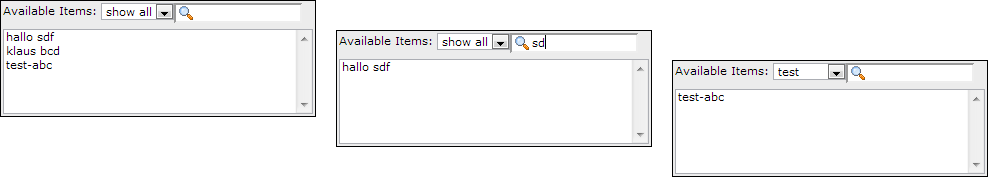
\includegraphics[width=1\linewidth]{Images/InDepthChanges/MultipleValueSelector.png}
	\end{figure}

\end{frame}

% ------------------------------------------------------------------------------
% Improved caching framework by introducing cache groups
% (slide added in March 2014)
% ------------------------------------------------------------------------------
% http://forge.typo3.org/issues/54991

\begin{frame}[fragile]
	\frametitle{Changements en profondeur}
	\framesubtitle{Groupes de cache (1)}

	\begin{itemize}
		\item Le cœur de TYPO3 utilise deux types de caches :

			\begin{itemize}
				\item \textbf{caches apparenté au système} :
				class loading cache, configuration cache, l10n\_cache, extbase\_object, extbase\_reflection etc.
				\item \textbf{caches apparenté au Frontend} :
				cHash cache, page cache, page section cache
			\end{itemize}

		\item Dans TYPO3 < 6.2, \textit{vider tous les caches} supprime \underline{tous} les caches, ce qui n'est pas optimal

		\item Dans TYPO3 >= 6.2, le cœur utilise deux groupes de cache :\newline
			« \textbf{pages} » regroupant tous les caches apparentés aux pages et\newline
			« \textbf{system} », utilisé pour les caches de compilation et de configuration

	\end{itemize}

	\begin{figure}
		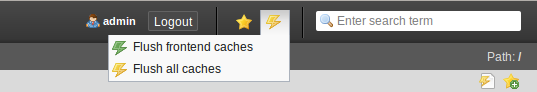
\includegraphics[width=0.5\linewidth]{Images/InDepthChanges/CacheGroups.png}
	\end{figure}

\end{frame}

% ------------------------------------------------------------------------------
% Improved caching framework by introducing cache groups
% (slide added in March 2014)
% ------------------------------------------------------------------------------
% http://forge.typo3.org/issues/54991

\begin{frame}[fragile]
	\frametitle{Changements en profondeur}
	\framesubtitle{Groupes de cache (2)}

	\lstset{
		basicstyle=\tiny\ttfamily
	}

	\begin{itemize}

		\item Option de configuration pertinente :\newline
			\smaller(dans les fichiers : \texttt{LocalConfiguration.php}/\texttt{DefaultConfiguration.php})\normalsize

			\begin{lstlisting}
			'cache_hash' => array(
			  'frontend' => 'TYPO3\CMS\Core\Cache\Frontend\VariableFrontend',
			  'backend' => 'TYPO3\CMS\Core\Cache\Backend\Typo3DatabaseBackend',
			  'options' => array(),
			  'groups' => array('pages', 'all')
			),
			\end{lstlisting}

		\item La commande « \textit{Purger tous les caches} » ne purge plus les caches apparentés au système (seul « Vider le cache de configuration » ou l'Install Tool vide ces caches)
		\item Une nouvelle option userTSconfig permet aux non-admins de vider les caches système :\newline
			\smaller\texttt{options.clearCache.system = 1}\normalsize

		\breakingchange

	\end{itemize}

\end{frame}

% ------------------------------------------------------------------------------
% TCA: limit number of ticked checkboxes
% (slide added in March 2014)
% ------------------------------------------------------------------------------
% http://forge.typo3.org/issues/55187
% http://forge.typo3.org/issues/55188 (documentation: TCA reference)

\begin{frame}[fragile]
	\frametitle{Changements en profondeur}
	\framesubtitle{TCA : Nombre de cases à cocher activées}

	\lstset{
		basicstyle=\tiny\ttfamily
	}

	\begin{itemize}
		\item TCA permet de contrôler le nombre de cases à cocher activées

			\begin{itemize}
				\item \texttt{maximumRecordsChecked} :\newline
					limiter le nombre de cases cochées globalement
				\item \texttt{maximumRecordsCheckedInPid} :\newline
					limiter le nombre de cases cochées par page (parente)
			\end{itemize}

		\item Si un utilisateur BE dépasse le nombre maximum, l'activation en trop s'annule jusqu'à ce qu'une autre case à cocher soit désactivée

		\item Exemple :

			\begin{lstlisting}
				$tcaConfiguration = array(
				  'type' => 'check',
				  'eval' => 'maximumRecordsChecked',
				  'validation' => array(
				    'maximumRecordsChecked' => 5
				  )
				);
			\end{lstlisting}

	\end{itemize}

\end{frame}

% ------------------------------------------------------------------------------
% TCA: Introduce MM_oppositeUsage property
% (slide added in March 2014)
% ------------------------------------------------------------------------------
% http://forge.typo3.org/issues/56061
% http://forge.typo3.org/issues/56123 (documentation: TCA reference)

\begin{frame}[fragile]
	\frametitle{Changements en profondeur}
	\framesubtitle{TCA : propriété \texttt{MM\_oppositeUsage}}

	\lstset{
		basicstyle=\tiny\ttfamily
	}

	\begin{itemize}
		\item Lors de la copie d'un enregistrement \texttt{sys\_category}, une nouvelle référence MM est créée, mais sans paramétrage du champ « fieldname »
		\item Cette valeur est définie depuis l'entité opposée de la relation à l'aide de \texttt{MM\_match\_fields}, mais ne peut être accédée
		\item Pour résoudre ce défaut, la nouvelle propriété \texttt{MM\_oppositeUsage} a été introduite pour le TCA :

			\begin{lstlisting}
				'config' => array(
				  'allowed' => '*',
				  'MM' => 'tx_myextension_first_second_mm',
				  'MM_oppositeUsage' => array(
				    'tt_content' => array('somefield'),
				    'tx_myextension_domain_model' => array('some_property'),
				  ),
				),
			\end{lstlisting}

	\end{itemize}

\end{frame}

% ------------------------------------------------------------------------------
% Miscellaneous
% ------------------------------------------------------------------------------
% http://forge.typo3.org/issues/49037 (Custom record list in element browser)
% http://forge.typo3.org/issues/36505 (Increase size of be_groups.subgroup field)
% http://forge.typo3.org/issues/49270 (Merge extensions TS/Template)

\begin{frame}[fragile]
	\frametitle{Changements en profondeur}
	\framesubtitle{Autres (1)}

	\begin{itemize}

		\item \textbf{Liste d'enregistrements personnalisée :}\newline
			\small
				Une liste d'enregistrements personnalisée peut être utilisée dans le navigateur d'élément pour surcharger celle fournie par défaut
			\normalsize

		\item \textbf{Plus de sous-groupes :}\newline
			\small
				L'attribut \texttt{subgroup} dans la table de la BD \texttt{be\_groups} est passée de \texttt{varchar(250)} à \texttt{text}, ce qui permet d'avoir beaucoup plus de sous-groupes (groupes d'utilisateurs Backend)
			\normalsize

		\item \textbf{Les extensions TS/Template ont été fusionnées :}\newline
			\small
				Techniquement, « WEB > Template » est composé de plusieurs extensions (tstemplate\_ceditor, tstemplate\_info,
tstemplate\_objbrowser et tstemplate\_analyzer). Ces extensions sont maintenant fusionnées en une seule extension : « tstemplate »
			\normalsize

	\end{itemize}
	
\end{frame}

% ------------------------------------------------------------------------------
% Miscellaneous
% ------------------------------------------------------------------------------
% http://forge.typo3.org/issues/49721 (Add label_userFunc_options support to BackendUtility)
% http://forge.typo3.org/issues/50441 (Add a timestamp when downloading an extension)
% http://forge.typo3.org/issues/51352 (Force saltedpasswords for Backend)

\begin{frame}[fragile]
	\frametitle{Changements en profondeur}
	\framesubtitle{Autres (2)}

	\begin{itemize}

		\item \textbf{label\_userFunc\_options :}\newline
			\small
				Le support de \texttt{label\_userFunc\_options} est ajouté à \texttt{BackendUtility}
			\normalsize

		\item \textbf{Nom du fichier d'extension :}\newline
			\small
				Lors du téléchargement d'une extension depuis le gestionnaire d'extensions, le nom du fichier contient un horodatage (année, mois, jour et heure) :\newline
				\texttt{<extensionKey>\_<version>\_<timestamp>.zip}\newline
				\texttt{monextension\_1.0.0\_201312102359.zip}
			\normalsize

		\item \textbf{EXT:saltedpasswords :}\newline
			\small
				L'extension EXT:saltedpasswords est une extension système requise et désormais activée par défaut.
				Cela force le salage pour l'authentification Backend. L'Install Tool vérifie les paramètres et les ajuste au besoin.
			\normalsize

	\end{itemize}
	
\end{frame}

% ------------------------------------------------------------------------------
% Miscellaneous
% ------------------------------------------------------------------------------
% http://forge.typo3.org/issues/51138 (Allow SignalSlots to modify arguments)
% http://forge.typo3.org/issues/31996 (Transfer query parameters in preview)

\begin{frame}[fragile]
	\frametitle{Changements en profondeur}
	\framesubtitle{Autres (3)}

	\begin{itemize}

		\item \textbf{Modification des arguments des SignalSlots :}\newline
			\small
				Les arguments passés au dispatcher de \textsf{SignalSlots} peuvent maintenant être modifiés et celui-ci retourne les arguments (modifiés) comme il les reçoit afin de garder l'enchaînement intact.
			\normalsize

		\item \textbf{Prévisualisation des espaces de travail :}\newline
			\small
				Les paramètres de requêtes sont désormais passés à la prévisualisation d'un espace de travail. Il y avait un problème sur TYPO3 < 6.2, les extensions qui passaient des paramètres personnalisés ne fonctionnaient pas correctement.
			\normalsize

		\item \textbf{Fonctionnalité TCEforms PlaceHolder :}\newline
			\small
				Introduite dans TYPO3 CMS 4.7, la fonctionnalité PlaceHolder des TCEforms fonctionne maintenant récursivement (ex. \texttt{\_\_row|uid\_foreign|field}).
			\normalsize

	\end{itemize}
	
\end{frame}

% ------------------------------------------------------------------------------
% Miscellaneous
% ------------------------------------------------------------------------------
% http://forge.typo3.org/issues/14730 (Support for proxy NTLM authentication)
% http://forge.typo3.org/issues/49667 (Enable double-resolution icons in SpriteGenerator)

\begin{frame}[fragile]
	\frametitle{Changements en profondeur}
	\framesubtitle{Autres (4)}

	\begin{itemize}

		\item \textbf{Icônes en double résolution :}\newline
			\small
				SpriteManager supporte désormais les icônes en haute résolution : il génère un second \textsf{Sprite} avec des dimensions doublées (un second fichier avec pour suffixe « @x2.png »). CSS3 assure qu'un fichier en haute résolution est chargé sur les appareils qui le supportent\newline
				(cela n'affecte pas les performances sur les autres appareils).
			\normalsize

		\item \textbf{Proxy avec authentification NTLM :}\newline
			\small
				Le support des proxys avec authentification NTLM (\textbf{NT} \textbf{L}AN \textbf{M}anager : ensemble de protocoles de sécurité de Microsoft) est ajouté. Cette fonctionnalité peut être activée dans l'Install Tool :\newline
			\normalsize			
				\texttt{\$GLOBALS['TYPO3\_CONF\_VARS']['SYS']['curlProxyNTLM']}\newline
				\emph{(par ailleurs, cette fonctionnalité a été demandée il y a plus de 8 ans :-)}
			\normalsize

	\end{itemize}
	
\end{frame}

% ------------------------------------------------------------------------------
% Miscellaneous
% (slide added in March 2014)
% ------------------------------------------------------------------------------
% http://forge.typo3.org/issues/14730 (Support for proxy NTLM authentication)

\begin{frame}[fragile]
	\frametitle{Changements en profondeur}
	\framesubtitle{Autres (5)}

	\begin{itemize}

		\item \textbf{cookieHttpOnly par défaut :}\newline
			\small
				Pour rendre le cookie de session uniquement accessible à travers le protocole HTTP, \texttt{cookieHttpOnly} est désormais activé par défaut.\newline
				Cela signifie que les cookies « fe\_typo\_user » et « be\_typo\_user » ne seront pas accessibles aux langages de scripts (par exemple JavaScript), ce qui durcit la protection contre les attaques XSS (\textit{cross site scripting}). D'ailleurs, certains anciens navigateurs ne supportent pas cette technique.
			\normalsize

		\item \textbf{Nettoyage de table en base de données :}\newline
			\small
				Les attributs suivants ont été retirés de la table \texttt{tt\_content} (non utilisé depuis TYPO3 4.0) :
				\texttt{text\_align}, \texttt{text\_face}, \texttt{text\_size}, \texttt{text\_color}, \texttt{text\_properties}.
			\normalsize

	\end{itemize}
	
\end{frame}

% ------------------------------------------------------------------------------
% Miscellaneous
% (slide added in March 2014)
% ------------------------------------------------------------------------------
% https://forge.typo3.org/issues/55190 (Move Tidy functionality to a TER extension)

\begin{frame}[fragile]
	\frametitle{Changements en profondeur}
	\framesubtitle{Autres (6)}

	\begin{itemize}

		\item \textbf{Retrait de « HTML Tidy » :}\newline
			\small
				La fonctionnalité \textit{HTML Tidy} a été retirée du cœur de TYPO3. Il peut facilement être remis en place en installant EXT:tidy depuis le TER.
			\normalsize

		\item \textbf{Retrait de « dontSetCookie » :}\newline
			\small
				Du fait que le cookie « fe\_typo\_user » est installé seulement s'il est requis (et pas toujours), l'option de l'Install Tool \texttt{dontSetCookie} devient inutile et a donc été retirée.
			\normalsize

		\item \textbf{Retrait des scripts « Wizard » :}\newline
			\small
				Suppression des scripts « wizard » suivants :
				\texttt{typo3/wizard\_add.php}, \texttt{typo3/wizard\_colorpicker.php}, \texttt{typo3/wizard\_edit.php}, \texttt{typo3/wizard\_forms.php}, \texttt{typo3/wizard\_list.php}, \texttt{typo3/wizard\_rte.php}, \texttt{typo3/wizard\_table.php}
			\normalsize

	\end{itemize}
	
\end{frame}

% ------------------------------------------------------------------------------

